\section{Auswahl der Trainingsinfrastruktur}

Bei der Auswahl der Trainingsinfrastruktur wurden zunächst die Cloud PaaS-Angebote in Betrachtung gezogen. Diese ermöglichen meist eine weit bessere Performance als lokales Training. Wichtig bei der Auswahl war hierbei möglichst niedrige Betriebskosten, ein diverses Angebot an Hardware-Beschleunigern und ein einfaches Aufsetzen der Trainingsinfrastruktur. Insbesondere sollten die Testversionen der jeweiligen Angebote zu Nutze gemacht werden. 

\textit{Amazon SageMaker} bietet hierbei für 50 Stunden eine \textit{ml.m4.xlarge} Instanz für Modelltrainingszwecke an \cite{AmazonWebServices.2020}. Da diese allerdings nur 4 vCPUs und 16 GiB Arbeitsspeicher umfasst, also keinerlei Cloud GPU als Hardwarebeschleuniger angeboten wird, wurde das Angebot wieder verworfen \cite{AmazonWebServices.20200314b}.

Auf Empfehlung wurde anschließend die \textit{GCP} betrachtet. Diese bietet mit 300\$ Startguthaben für 12 Monate ein lukratives Angebot zum Ausprobieren von beliebigen \textit{GCP} Produkten \cite{GoogleCloudPlatform.20200314b}. Die Benutzung der \textit{Deep Learning VM} bietet zudem eine native Unterstützung des \textit{PyTorch} Frameworks, was von der \textit{SSD} Implementierung genutzt wird, und zugleich eine Auswahl aus vier gängigen Cloud GPUs, der \textit{NVIDIA Tesla K80}, \textit{NVIDIA Tesla P100}, \textit{NVIDIA Tesla T4} und der \textit{NVIDIA Tesla V100}. Um die Konfiguration der \textit{Deep Learning VM} allerdings mit Auswahl einer Cloud GPU abschließen zu können, muss zunächst das mit dem Account verknüpfte Kontingent erhöht werden. Hierzu konnte an das \textit{GCP} Support Team ein offizieller Antrag gestellt werden. Aufgrund der geringen Kaufhistorie wurde der Antrag allerdings abgelehnt. 

\textit{Microsoft Azure} bietet für 200\$ bei einer Laufzeit von 30 Tagen Zugang zu allen \textit{Microsoft Azure} Diensten \cite{MicrosoftAzure.2020}. Darunter gehört eine \textit{NC6} Instanz mit sechs vCPUs und einer \textit{NVIDIA Tesla K80} \cite{MicrosoftAzure.202003124}. Da \textit{Microsoft Azures} Angebot allerdings nur sehr oberflächlich beschrieben wurde, wurde sich letzten Endes auch gegen \textit{Microsoft Azure} entschieden. 

Als letzter Anbieter wurde \textit{FloydHub} getestet. Hervorzuheben ist die besonders einfache Vorgehensweise bei der Account Erstellung und dem Aufsetzen der Trainingsinfrastruktur, was bereits im Grundlagen Kapitel beschrieben wurde. \textit{FloydHub} bietet 20 Stunden CPU Trainingszeit bzw. 2 Stunden GPU Trainingszeit auf einer \textit{NVIDIA Tesla K80} \cite{FloydHub.2020}. Neben einer \textit{NVIDIA Tesla K80} konnte ebenso Trainingszeit auf einer \textit{NVIDIA Tesla V100} erworben werden. Zudem wurde das verwendete \textit{PyTorch} Framework unterstützt. Aufgrund der einfachen Handhabung wurde sich trotz der erhöhten Kosten für \textit{FloydHub} entschieden. 

Während des Trainings mit der \textit{NVIDIA Tesla K80} fiel allerdings auf, dass die Wahl dieser GPU keine großen Performance Verbesserungen brachte. Dies veranlasste eine Gegenüberstellung gängiger Cloud GPUs mit lokalen GPUs, allen voran den bereits vorhandenen Desktop-Grafikkarten \textit{GeForce GTX 1080} und \textit{Titan RTX} \ref{gpus} \cite{TechPowerUp.20200209}.

\begin{center}
	\begin{tabular}[h]{l|c|c|c|c|c|c}
		& K80 & P100 & T4 & V100 & GTX 1080 & TITAN RTX \\
		\hline
		CUDA Cores & 2496 & 3584 & 2560 & 5120 & 2560 & 4608 \\
		Tensor Cores & / & / & 320 & 640 & / & 576 \\
		TeraFLOPS (Single Precision) & 4,113 & 9,526 & 8,141 & 14,13 & 8,873 & 16,31 \\
		Memory Bandwidth (in GB/sec) & 240,6 & 732,2 & 320 & 897 & 320,3 & 672 \\
		Suggested Power Supply Unit & 700 & 600 & 350 & 600 & 450 & 600
		\label{gpus}
	\end{tabular}
	\captionof{table}{Vergleich von GPUs nach Rechenleistung}
\end{center}

Hierbei fällt auf, dass im Grad der Parallelisierung eine \textit{NVIDIA Tesla K80} zwar mit den vorhandenen lokalen Grafikkarten mithalten kann, in der Anzahl an Rechenoperationen pro Sekunden allerdings weit schlechter abschneidet. Damit sich das Training in der Cloud nach Performance lohnt, muss demnach mindestens eine \textit{NVIDIA Tesla V100} verwendet werden. Da diese allerdings mit 42\$ für zehn Stunden mehr als dreimal so teuer wie eine \textit{NVIDIA Tesla K80} für 12\$ ist und zusätzlich zu den GPU Kosten noch monatliche Account-Gebühren berechnet werden\footnote{Je nach Account kann eine unterschiedliche Anzahl an Projekten erstellt und Speicherplatz verwendet werden. Die \textit{Beginner} Ausstattung von einem Projekt und 10 GB Speicher ist allerdings kostenfrei.}, wurde sich nach nun nach Kosten-Nutzen Abwägung letzten Endes auf lokales Training festgelegt. Dies ist ebenso hinsichtlich des Trainings des \textit{YOLO} Objektdetektors besser, da das sehr spezifische \textit{Darknet} Framework, das in der Implementierung genutzt wird, bisher von noch keinem Cloud Anbieter unterstützt wurde. Dies hätte eine Umentscheidung auf eine Alternativ-Implementierung in beispielsweise \textit{TensorFlow} oder \textit{PyTorch} nötig gemacht.

Auch wurden Überlegungen zum Training in \textit{Google Colab} unternommen, da diese einfach ein Training mit TPUs ermöglichen. Diese Art von Spezialhardware erreicht pro TPU-Kern eine Rechenleistung von bis zu 92 TOPS \cite{HaraldBogeholz.20170406}. Werden 2048 solcher TPU-Kerne zu einem TPU-Pod zusammen geschlossen, so ergibt sich eine Rechenleistung von über 100 PetaFLOPS \cite{GoogleCloud.20200209}. Zudem ist die größere Rechenleistung gleichzeitig effizienter als herkömmliche GPUs (siehe Abbildung \ref{tpu}).

\begin{figure}[ht]
	\begin{center}
		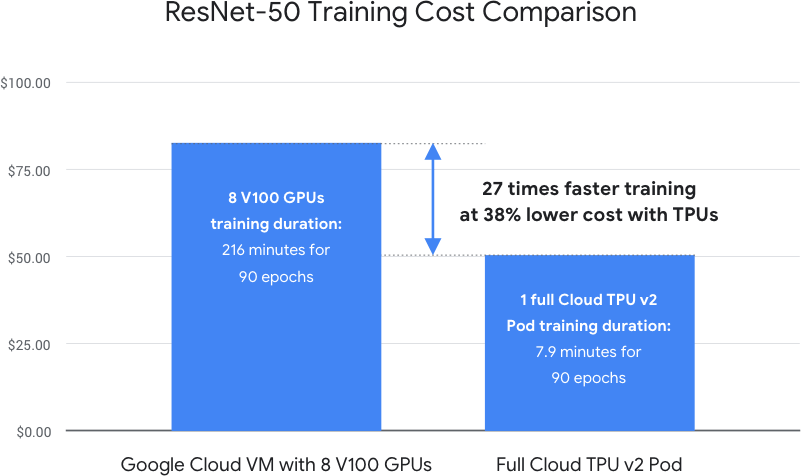
\includegraphics[width=14cm]{Bilder/tpu_comparison.png} 
		\caption[Vergleich V100 - TPU Pod]{Vergleich V100 - TPU Pod \cite{GoogleCloud.20200209b}}
		\label{tpu}
	\end{center}
\end{figure}

Da allerdings in \textit{Google Colab} nach 90 Minuten ein Trainingsjob beendet wird und die Rechenresourcen neuen Nutzern zugewiesen werden, war diese Art des Trainings ebenfalls nicht möglich. 